\documentclass[11pt]{article}
\usepackage[utf8]{inputenc}
\usepackage{amsmath, amsthm, amssymb}
\usepackage[letterpaper, margin=1in]{geometry}
\usepackage{microtype}
\usepackage[shortlabels]{enumitem}
\usepackage{biblatex}
\usepackage{mathtools}
\usepackage{amssymb}
\usepackage{float}
\usepackage{commath}
\usepackage{color, soul}
\usepackage{wrapfig}
\usepackage{xfrac}
\usepackage{hyperref}
\usepackage[colorinlistoftodos,textsize=tiny]{todonotes}
\usepackage{comment}

\let\comment\todo
\newcommand{\frank}[1]{\comment[nolist,color=blue!40]{f: #1}}
\newcommand{\david}[1]{\comment[nolist,color=orange!40]{d: #1}}
\newcommand{\katie}[1]{\comment[nolist,color=green!40]{k: #1}}

\addbibresource{main.bib}

\newtheorem{theorem}{Theorem}[section]
\newtheorem{corollary}{Corollary}[theorem]
\newtheorem{lemma}[theorem]{Lemma}
\newtheorem{alg}[theorem]{Algorithm}
\newtheorem{claim}[theorem]{Claim}

\theoremstyle{definition}
\newtheorem{definition}{Definition}[section]

\theoremstyle{definition}
\newtheorem{subroutine}{Subroutine}

\theoremstyle{definition}
\newtheorem{example}{Example}[section]

% Commonly used symbols
\newcommand{\R}{\mathbb{R}}
\newcommand{\fu}{f^{\mu}}
\newcommand{\nfi}{\nabla f_i}
\newcommand{\nfiu}{\nabla \fu_i}
\newcommand{\biu}{b_{i}^{\mu}}
\newcommand{\gij}{\gamma_{ij}}
\newcommand{\geu}{\gamma_e^{\mu}}
\newcommand{\giij}{\gamma_{ij}^{\mu}}
\newcommand{\vnott}{V \setminus t}
\newcommand{\din}{\delta^{\text{in}}}
\newcommand{\dout}{\delta^{\text{out}}}
\newcommand{\vsrc}{V^{s}}
\newcommand{\vsink}{V^{t}}
\newcommand{\vz}{V^{0}}
\newcommand{\fp}{(f,\mu)}
\newcommand{\fiju}{f_{ij}^{\mu}}

\newcommand{\tf}{\textsc{Tight-Flow}}
\newcommand{\ppn}{\textsc{Produce-Plentiful-Node}}
\newcommand{\filtration}{\textsc{Filtration}}
\newcommand{\es}{\textsc{Elementary-Step}}

\newcommand{\xands}{X \cap S}
\newcommand{\xnots}{X \setminus S}
\DeclareMathOperator{\Ex}{Ex}
\DeclareMathOperator{\Def}{Def}

\newcommand{\rewrite}[1]{\textcolor{red}{#1}}
\renewcommand{\todo}[1]{\hl{TODO: #1}}

\newcommand{\lpeq}[1] {
\begin{equation*}
\begin{aligned}
#1
\end{aligned}
\end{equation*}
}
\newcommand{\lpone}[3] {
& \underset{}{\text{#1}}
&& #2 \\
& \text{s.t.}
&& #3 
}
\newcommand{\lptwo}[4] {
\lpone{#1}{#2}{#3}\\
&&& #4
}
\newcommand{\lpthree}[5] {
\lptwo{#1}{#2}{#3}{#4}\\
&&& #5
}

\title{Strongly Polynomial Algorithms for Generalized Flow Maximization}
\author{Francis Cangialosi, Katie Lewis, David Palmer}
\date{}

\begin{document}
\maketitle
\section{Introduction}\label{sec:intro}
	\subsection{Problem Definition}\label{sec:problem}
	As in the traditional flow problem, given a
	graph $G = (V,E)$, the generalized maximum flow problem aims to maximize the
	total flow delivered to the sink node $t \in V$. Unlike the original flow
	problem however, each edge contains a gain factor $\gamma_e > 0$, which scales
	the flow passing through that edge. Intuitively, this scaling can be thought
	of in terms of real world examples such as exchange rates between currencies
	or physical transformations due to energy dissipation. The generalized maximum
	flow problem lacks several nice properties that are present in the traditional
	maximum flow problem, which makes it more challenging to solve. For example,
	the generalized problem is usually thought to be non-integral and,
	due to the gain factors, the total supply is not necessarily equal to the total
	demand. Additionally, the maximum flow--minimum cut theorem no longer applies
	since the flow along a path is not equal at every edge along that path.
    
	Until recently, the best known algorithms were all weakly polynomial. In
	2013, Végh developed the first strongly polynomial algorithm~\cite{Vegh2013}
	(i.e. one that depends only on the number of nodes and edges in the graph,
	and is independent of the size of their values). In 2017, Olver and Végh
	built on this work and developed an algorithm~\cite{Olver2017}
    that is faster by a factor of
	almost $O(n^2)$, resulting in a running time that is as fast as the best
	weakly polynomial algorithms even for small parameter values. These
	algorithms take advantage of the structural similarities between the
	generalized maximum flow problem and the minimum cost flow problem by
	adapting techniques from well-known combinatorial min cost flow algorithms,
    namely~\cite{Orlin1988}.
    
	\subsection{Structure and Contributions of the Paper}\label{sec:structure}
	In this paper, we aim to
	familiarize the reader with the recent algorithmic developments for the
	generalized flow maximization problem and provide intuition for the techniques
	used to achieve a strongly polynomial result. In Section~\ref{sec:prelim}, we more formally
	define the problem as a linear program and give an overview of the notation
	used in the rest of the paper. In Section~\ref{sec:motivate}, we develop the key techniques
	shared by both algorithms used to achieve a strongly polynomial bound for this
	problem. In Section~\ref{sec:2013}, we describe Végh's original $O(n^3m^2 \log n)$ strongly
	polynomial algorithm developed in 2014 and present a more intuitive and
	detailed analysis than the original paper. In Section~\ref{sec:2017}, we describe Olver and
	Végh's faster $O((m + n\log n)mn\log(n^2 / m))$ algorithm and highlight key
	aspects of the analysis that led way to the improved running time efficiency.
	Finally, in Section~\ref{sec:discussion}, 
    \rewrite{we conclude with open questions and present a few ideas
	for future work.}
	\todo{Update when we're done.}
    
\section{Preliminaries}\label{sec:prelim}

	\subsection{Network Notation}\label{sec:notation}
	%An instance of the generalized flow problem is specified as	
	Let $G=(V,E)$ be a directed graph with $n=\abs{V}$ and $m=\abs{E}$,
	$t \in V$ be a sink node and $\gamma \in \R_{>0}^E$ be the vector of flow gains
	across the edges. Although we have typically seen flow constraints defined in terms of
	edge capacities, recent work on the generalized problem defines flow
	constraints using node demands $b \in \R^{V \setminus t}$ instead (and leave
	edge capacities unbounded). Thus, an instance of the generalized flow problem
	is specified as $(G, t, \gamma, b)$.
	We adopt this formulation in our paper for
	convenience of analysis. As shown in~\cite{Vegh2013}, any problem defined with
	node demands can be easily transformed to an equivalent problem with
	capacities (and vice versa). 

	Although there is no explicit specification of a source node, the concept of
	node demands generalizes the concept of having multiple sources and multiple
	sinks: nodes with negative demand $-b$ act as sources because they can create
	up to $b$ units of flow, and nodes with positive demand $b$ act as sinks 
	because they consume at least $b$ units of flow. Thus, (excluding $t$), we denote the subset of
	nodes with negative demand as $\vsrc$, the subset of nodes with positive
	demand as $\vsink$, and the remaining nodes with zero demand as $\vz$.

	For a subset of the nodes $S \subseteq V$, we define $\din(S)$ and
	$\dout(S)$ to be the set of incoming and outgoing edges, respectively,
	and let $d_i = |\din(\{i\}) \cup \dout(\{i\})|$ be the total degree of a
	node $i \in V$.

	Then we can define the net flow at a node $i$ as the amount of flow that
	reaches a node (scaled by the gain factor on the incoming edges) minus the
	amount of flow that leaves the node: 
	$$ \nfi \coloneqq \sum_{e \in \din(i)} \gamma_e f_e - \sum_{e \in \dout(i)} f_e.$$

	The residual graph $G_f = (V,E_f)$ is defined as in the traditional problem,
	except the reverse residual edges $(j,i) \in E_f$ have inverted gain 
	$\gamma_{ji} = 1 / \gamma_{ij}$ and negated flow $f_{ji} =
	-\gamma_{ij}f_{ij}$. If the cumulative gain of a cycle $C$ ($\prod_{e \in C} \gamma_e$)
	in $G_f$ is greater than 1, we call $C$ a ``flow-generating cycle.'' 
	This captures the idea of arbitrage: sending a unit of flow around the cycle
	generates a net surplus.





	\subsection{Linear Program Formulation}
	\label{sec:lp}

	We formulate the generalized flow maximization problem with demands as in the 2017
	paper~\cite{Olver2017}:
	\vspace{-0.35cm}
%		\begin{align*}
%		\text{max} \quad
%		\nabla f_t& \\
%		\text{s.t.} \quad \tag{P}
%		\nabla f_i &\geq b_i \quad \forall i \in V \setminus t \\
%		f &\geq 0
%		\end{align*}        
%
%		\noindent The dual of (P) is shown below on the left. If we set
%		\rewrite{$\mu = \mu$}, we arrive at the formulation on the right,
%		as given in~\cite{Olver2017}:
%

    \begin{align*}\tag{P}
    \text{max} \quad
    \nabla f_t& \\
    \text{s.t.} \quad
    \nabla f_i &\geq b_i \quad \forall i \in V \setminus t \\
    f &\geq 0
    \end{align*}

	The dual linear program, given on the left below, has a variable $\eta_i$ for
	every node $i$. 
	Making the change of variables $\eta_i = - \mu_t / \mu_i$ yields the
	dual optimization problem on the right.
    \vspace{0.5cm}

	\begin{tabular}{rcll}
		\hspace*{-1.05cm}
	\resizebox{0.37\textwidth}{!}{
		\fbox{
	\begin{minipage}{0.35\textwidth}
	\begin{alignat*}{4}
    \text{min} &\quad &\sum_{i \in V \setminus t} b_i \eta_i \\
    \text{s.t.}
    &   &\gij \eta_j - \eta_i &\geq 0 \quad &&\forall\; &&(i, j) \in E \\
    &   &                     &             &&          &&\ i, j \neq t \\
    &   &\gamma_{ti} \eta_i &\geq -1 \quad  &&\forall\; &&(i, t) \in E \\
    &   &-\eta_i &\geq \gamma_{it} \quad    &&\forall\; &&(t, i) \in E \\
    &   &\eta_i &\leq 0 \quad               &&\forall\; &&i \in V \setminus t
    \end{alignat*}
	\end{minipage}
}
} & 
	$\xrightarrow{\hspace*{0.25cm}\eta_i = - \mu_t / \mu_i\hspace*{0.25cm}}$
	&
	\resizebox{0.37\textwidth}{!}{
		\fbox{
	\begin{minipage}{0.4\textwidth}
    \begin{alignat*}{3}
    \text{max} &\quad &\mu_t &\sum_{j \in V \setminus t} \frac{b_j}{\mu_j}  \\
    \text{s.t.}
    &   &\gij \mu_i &\leq \mu_j \quad &&\forall\; (i, j) \in E \\
    &   &\mu_i &\in \R_{>0} \cup \infty \quad &&\forall\; i \in V \setminus t \\
    &   &\mu_t &\in \R_{>0}
    \end{alignat*}
	\end{minipage}
}
} & \hspace*{0.4cm}(D)
\end{tabular}
\vspace{0.5cm}

        
	A dual solution $\mu$ is known as a \emph{labeling}, and we can speak of feasible and
	optimal labelings. We make the simplifying assumption that the sink is
	reachable from every node, which ensures $\mu$ will be finite. (\cite{Olver2017} shows a simple transformation that allows us to guarantee this assumption.) 
	Complementary slackness requires that for an optimal flow $f^*$ and optimal labeling $\mu^*$,
    \begin{equation}\label{eqn.cs} \tag{CS}
    f^*_{ij} > 0 \implies \gamma_{ij}\mu^*_i = \mu^*_j.
    \end{equation}
	This suggests a particular interpretation of the dual variables. Imagine that
	the nodes represent currencies and the gains represent exchange rates between those currencies.
	A maximum generalized flow is the currency trading strategy that maximizes the value in currency
	$t$ at the end. We can interpret a label $\mu_i$ as the value of one dollar in currency $i$.
	The dual constraint $\gamma_{ij} \mu_i \leq \mu_j$ means that under the labeling $\mu$,
	it is not possible to create value by converting currencies.
	The complementary slackness condition means that the currency trading strategy
	only makes trades that exactly preserve value.
    \todo{Be sure to mention we assume no flow-generating cycles and
    why we can make this assumption (cancel them).}
	
    % $\mu$ is a value assignment. We're rewriting the problem in a different
		% currency. The relabeled dual problem is equiavelnt to the original dual
		% problem, the constraints for tight edges become replace $\mu$ with $\mu'$
		% in all the constraints. There's a dual problem which solves for $\mu'$ on
		% each node, and you can then get a solution to the original problem which is $\mu*\mu'$

	Given a feasible dual solution $\mu$, we can apply the following \textbf{relabeling}
    transformation to obtain a new problem instance with gains $\gamma^\mu$ and demands $b^\mu$
    and a primal solution to the new instance:
	\[ \gamma_{ij}^\mu \coloneqq \gamma_{ij} \frac{\mu_i}{\mu_j} \quad
	b_i^\mu \coloneqq \frac{b_i}{\mu_i} \quad
    f_{ij}^\mu \coloneqq \frac{f_{ij}}{\mu_i} \quad
	\nabla f_i^\mu \coloneqq \frac{\nabla f_i }{\mu_i} \]
    The relabeled dual problem is equivalent to the original dual problem. In particular,
    \begin{claim}
    $f^\mu$ is a feasible (resp. optimal) solution to the relabeled primal problem with gains
    $\gamma^\mu$ and demands $b^\mu$ if and only if $f$ is a feasible (resp. optimal) solution
    to the original problem with gains $\gamma$ and demands $b$. \katie{which original problem?}
    \end{claim}
    \begin{claim}
    If $\mu$ is a feasible solution to the original dual problem and
    $\bar{\mu}^*$ is an optimal solution to the relabeled dual problem with gains
    $\gamma^\mu$ and demands $b^\mu$,
    then the vertex-wise product $\mu\bar{\mu}^*$ is an optimal solution to the original dual problem.
    \end{claim}
    We will often use relabeling to simplify the problem while preserving its structure.\todo{maybe revisit this and condense / simplify more}
    
    \begin{definition} \label{def.tight}
	An edge $e$ is known as \textbf{tight} with respect to $\mu$ if $\gamma_e^\mu =1$.
	For an optimal pair $(f, \mu)$, complementary slackness is exactly the condition that
	flow only flows along tight edges. We denote the set of tight edges under
	$\mu$ by
    \[ \tau(\mu) = \{e \mid \geu = 1\}. \]
    The \textbf{tight graph} consists of these edges and their endpoints.
	\end{definition}
    
	Given flow values and labels, the total excess and deficit of the flow with respect
	to the labels is defined as follows:
	\begin{align*}
	\Ex(f,\mu)  &\coloneqq \sum_{i \in V \setminus t} \max \{ \nfiu - \biu, 0 \} \\
	\Def(f,\mu) &\coloneqq \sum_{i \in V \setminus t} \max \{ \biu - \nfiu, 0 \}
	\end{align*}
  
\section{Motivating Ideas and Techniques}
\label{sec:motivate}
	\subsection{Solving the Dual Problem Combinatorially}
	\label{sec:motivate-dual}
    	%* Talk about idea of solving dual 
      %  	* Key insight about this algorithm is that they maintain $f^{\mu}$ (without any extra work apparently) to be integral
      %      * Allows normal flow algorithms 
      %      * Is maintaining solution that is "close enough to feasible primal" with complementary slackness unique to this algorithm?
      %      * Draw parallels between min cost flow and generalized max flow (give more clear and intuitive explanation than the Truemper paper)
	
	A weakly polynomial algorithm is easily achievable by applying ellipsoid or
	interior point methods to the linear program (P). To achieve a strongly polynomial
	bound, the linear program must be reduced to a more combinatorial problem.
	
	Both algorithms discussed below employ a simple (and strongly polynomial)
	reduction to the dual problem (D).
    Given optimal dual labels $\mu$, consider the primal problem relabeled by $\mu$.
    Complementary slackness dictates that for any optimal flow $f$,
    $\giij = \gij\mu_i/\mu_j = 1$ whenever $f_{ij} > 0$. As such, the conservation
    constraint for the relabeled optimum flow $f^\mu$ takes the form
    \[ b^{\mu} \leq \nabla f^{\mu}
    = \sum_{j \in \din(i)} \giij \fu_{ij} - \sum_{j \in \dout(i)} \fu_{ji}
    = \sum_{j \in \din(i)} \fu_{ij} - \sum_{j \in \dout(i)} \fu_{ji}. \]
    This is the conservation constraint of an ordinary maximum flow problem with demands
    $b^\mu$, and indeed one can compute the optimal $f^\mu$ as an
    ordinary maximum flow on the tight graph---a strongly polynomial operation.
    Then it is easy to recover $f$ from $f^\mu$.
    
    In fact, modulo an ordinary maximum flow computation, the dual problem reduces to computing the set of tight edges.
		\todo{Is think we should clarify this. What is \textit{the} set of tight edges?}
    Since regular maximum
    flow has already been solved in strongly polynomial time, it suffices to find a strongly polynomial
    algorithm to compute a set of tight edges consistent with a dual optimal solution. This problem
    is inherently combinatorial, suggesting that it can be solved in strongly polynomial time.
    
    \subsection{Contracting edges}\label{sec:contract}
    To organize the search for tight edges, both algorithms inductively reduce the graph.
    Suppose an edge $(i, j)$ is known to be tight for any dual-optimal solution $\mu$. This
    imposes a constraint $\giij = 1$ for all such $\mu$, or, i.e., $\gij \mu_i = \mu_j$.
    Imposing a constraint of this form reduces the dimension of the solution
    space by one and is equivalent to removing one variable from optimization. Indeed,
    suppose we solve the equivalent problem instance $(\biu, \giij)$. Then the new constraint
    becomes $\mu_i' = \mu_j'$. In order to avoid working with extra constraints, we might
    as well remove one of the variables entirely by collapsing the edge $(i, j)$, leaving a single
    node $j$ with a single dual variable $\mu_j$. It remains to set the demand $b_j$ so
    that the problem remains equivalent. Rewritten in terms of the variables in
    the modified problem, the relevant terms of the dual objective are
    \[ \mu_t' \left(\frac{b_i^\mu}{\mu_i'} + \frac{b_j^\mu}{\mu_j'}\right)
     = \mu_t' \left(\frac{b_i^\mu + b_j^\mu}{\mu_j'}\right). \]
	So the operation of collapsing $i$ into $j$ along $(i, j)$ and summing their demands
	preserves the objective and constraints.
	
	We can make one additional simplification: if the contraction leads to parallel edges,
	only the one with the highest gain is maintained. This is motivated by the primal problem: in
	the absence of edge capacity constraints, there is no reason to send flow along an edge of
	lower gain when one of higher gain is available. Thus, culling parallel edges preserves the
	essential features of the problem.
	
	\subsection{Progress}

	%Following from the previous two sections, in order to optimize the dual,
	%both algorithms make progress by alternating between finding contractible
	%edges and contracting them.
	The heart of both strongly polynomial algorithms is a procedure for
	identifying contractible edges and then contracting them. The key
	differences between the two algorithms are in 
	\textit{how} they find contractible edges, which
	we will describe in Sections~\ref{sec:2013} and~\ref{sec:2017}. These differences
	allow Olver and Végh \cite{Olver2017} to achieve a better running time bound than
	Végh \cite{Vegh2013}.

	Contractions continue until one of the following cases occurs:
	\begin{enumerate}[(i)]
	\item the contracted graph has just one node remaining, i.e., every node has been merged
	into the sink $t$. In this case, the set of previously identified
	contractible edges forms a spanning tree. Given a value for $\mu_t$, the tightness
	constraints then uniquely determine the values of the optimal $\mu$ at all other vertices.
	
	\item the contracted graph has multiple nodes, but the (merged)
	demands $\biu$ are all zero. In this case, the dual objective on the contracted
	graph is identically zero, and the primal solution $f \equiv 0$ is feasible,
	with a primal objective value of zero. By strong duality, any feasible dual
	solution on the contracted graph is optimal---in particular, the feasible
	solution produced during the contractions is optimal.
	In this case, the set of contractible edges
	forms a spanning forest where each component is identified with one node
	of the contracted graph. Given the values of the dual solution at these vertices,
	the tight spanning forest provides a recipe for reconstructing
	an optimal dual over the original graph.
	
	From the primal perspective, each component of the tight forest has net ($\mu$-relabeled)
	demand zero. As such, the flows in separate components are independent, and the objective
	value only depends on the flow on the tight tree component containing the sink $t$.
	As observed in Section \ref{sec:motivate-dual}, this
	can be computed (in strongly polynomial time)
	by an ordinary maximum flow computation over the edges of the tight tree containing $t$.
	\end{enumerate}
    
    \begin{example}
    Consider the simple flow network in
    Figure~\ref{fig:ex-graph}. \ By inspection, we can see that the maximum flow $f^{*}$
    should send 8 units of flow along the top edge and 8 units of flow along the bottom edge,
    resulting in 6 units at the sink. In Figure~\ref{fix:ex-spanning},
    we show the three possible tight spanning trees for this graph.
    In (a), the dual is not feasible. (b) and (c) are both feasible,
    but the value produced by (c) is greater, and is thus optimal.
    \end{example}


\section{The Initial Strongly Polynomial Algorithm}
	\subsection{Introduced Concepts and Notation}
    \label{sec:2013-notation}

%Notes for "Intuitive Section 4":

%-continuous scaling -> find contractible edges -> optimal dual -> optimal primal
%-continuous scaling -> breaks down usual $\Delta$ phases so won't over-shoot labeling
%-maintain feasible primal solution by keeping $\Delta$-feasible pair -- ensures security reserve $e_i >= R_i$
%-maintain bound on excess for individual nodes
%-trying to minimize max excess -- why?
%-push flow/excess around to create/identify abundant arc $(f_ij) >= 17m\Delta$
%-nodes with relabeled b magnitude $>= 20mn\Delta$ must have abundant arc adjacent
%-Pushes excess around by augmenting and relabeling; if algorithm gets "stuck", uses filtration to push flow around and even out excess in an "isolated" part of graph (not part of frontier)
%-algorithm maintains that b/delta is non-decreasing
%-cycle canceling only once in beginning -- explain why and assumptions?


Végh's initial algorithm \cite{Vegh2013} was the first strongly polynomial algorithm for the generalized flow maximization problem. This algorithm achieves a strongly polynomial runtime by improving upon scaling techniques used in previous weakly polynomial algorithms such as FAT-PATH \cite{Goldberg:1991:CAG:105014.105022} and also by integrating the concepts of abundant and contractible edges from Orlin's minimum cost flow algorithm \cite{Orlin1988}. 

Orlin's \textit{abundant arc} concept can be applied to generalized max flow to show that if an edge has a large amount of flow in comparison to the value of the scaling factor $\Delta$, then that edge must have non-zero flow in the primal solution and, by complementary slackness, the edge must be tight in every dual solution. Therefore that edge can be contracted as shown in Section~\ref{sec:contract}. At a high-level, Végh's generalized max flow algorithm maintains a feasible primal solution while trying to identify these contractible edges to find an optimal dual solution. Once found, the optimal dual solution can be used to easily transform the feasible primal solution to an optimal primal solution via one traditional max flow iteration as shown in Section~\ref{sec:motivate-dual}.

In order to find contractible edges in strongly polynomial time, this algorithm introduces the concept of \textit{continuous scaling}. Previous scaling algorithms for this problem use distinct $\Delta$-scaling phases, where $\Delta$ is only updated after a constant number of path augmentations. This can cause an ``over-shooting'' problem in which $\Delta$ increases too quickly relative to $f^\mu$ to guarantee abundant edges. As a solution, this algorithm continuously alternates between augmenting $\Delta$ units of flow from ``high-excess'' nodes to ``low-excess'' nodes (including the sink) and proportionately increasing $\mu$ and decreasing $\Delta$. Since $\Delta$ and $\mu$ are always scaled coherently, their relative magnitude stays bounded and non-decreasing, which addresses the over-shooting problem.
\label{sec:2013}
	
	This algorithm employs scaling parametrized by a factor $\Delta$.
    \begin{definition}
	For $\Delta \geq 0$, the \textbf{$\Delta$-fat graph} consists of all
	forward edges $(i, j)$ and those reverse edges $(j, i)$ with $f_{ij}^\mu > \Delta$. This
    is the portion of the residual graph with at least $\Delta$ capacity.
    \end{definition}
    Végh's initial strongly polynomial algorithm \cite{Vegh2013}
	introduces the notion of a \textit{conservative labeling}, which helps to
	identify the highest gain augmenting paths on which to push flow.
	\begin{definition}
	$\mu$ is a \textbf{conservative labeling} for $f$, a feasible solution to (P), if $\mu$ is
	a feasible solution to (D) and all edges with positive flow are tight.
	\end{definition}
    \begin{definition}
    $\mu$ is a $\Delta$-conservative labeling for $f$, or alternatively $(f, \mu)$ are a
	$\Delta$-feasible pair, if
        \begin{enumerate}[(i)]
        \item $f_{ij}^\mu \leq \Delta$ for all non-tight edges $(i, j)$;
        \item $\mu_t = 1$; and
        \item $\mu_i > 0, \nfi - b_i \geq R_i$ for all $i \in V \setminus t$ where $R_i$ is the total incoming flow on non-tight edges
        \end{enumerate}
   \end{definition}
    
	The scaling algorithm aims to identify \emph{contractible} edges,
	edges that are tight in every optimal dual solution,
    in a strongly polynomial number of steps. This technique was
    originally developed to study the minimum cost flow problem (\emph{cf.}~\cite{Orlin1988}). \todo{need to define this or refer to section 3?}
	As we will show in Section~\ref{sec:cert} Lemma~\ref{lem.contractibility}, a large flow value along an edge can
    serve as a certificate of contractibility. To that end, we define
    \begin{definition}
    An edge $(i, j)$ is \textbf{abundant} at scale $\Delta$ if $f_{ij}^\mu \geq 17m\Delta$.
    \end{definition}
		\todo{At least give intuition for how they derived this number}
	Once the algorithm identifies an abundant edge,
	it can contract the edge and reduce the size of the graph. The algorithm
	terminates once the graph reduces to one node; this leads to a
	strongly polynomial bound on the number of iterations of this algorithm.

This algorithm also extends the scaling technique in the FAT-PATH algorithm
    \cite{Goldberg:1991:CAG:105014.105022} by introducing \textit{continuous scaling}. At a high-level, the continuous scaling
    method alternately (i) augments $\Delta$ units of flow along a tight path from high
    excess nodes to low excess nodes (including the sink) or (ii) proportionately increases $\mu$ and
    decreases $\Delta$. Unlike previous scaling methods used for the generalized flow problem, such as FAT-PATH \cite{Goldberg:1991:CAG:105014.105022},
    this algorithm does not have distinct $\Delta$-phases; instead, $\Delta$ is updated continuously.
    
    As $\Delta$ and $\mu$ are always scaled coherently, their relative magnitude will stay bounded.
    This addresses an ``over-shooting'' problem common in previous scaling algorithms in which $\Delta$
    increases too quickly relative to $f^\mu$ to guarantee abundant edges.
    
    As $\Delta$ changes, the algorithm maintains a $\Delta$-feasible pair, which ensures that there is
    a ``reachable'' feasible solution to (P). If $(f,\mu)$ is a $\Delta$-feasible pair,
    setting the flow on non-tight edges to zero yields a feasible pair.
    Given this, the algorithm only needs to run a cycle-canceling
    algorithm once on the initial solution and then feasibility is maintained throughout the rest of
    the algorithm.
    
	\subsection{Algorithm Overview} \label{sec:2013-overview}
	%\begin{table}[H]
	%\begin{center}
	%    \begin{tabular}{ | p{7cm} | p{7cm} |}
	%    \hline
	%    Challenges in Previous Algorithms  & Solutions from Algorithm \\ \hline
	%    ``Abundant edge'' might not appear in strongly polynomial number of steps \cite{Radzik2004} & Continuous Scaling Method  \\ \hline
	%    Augmentation along highest gain paths introduce flow generating cycles; must run cycle-canceling algorithms in every scaling phase \cite{Goldberg:1991:CAG:105014.105022} & Maintain a $\Delta$-conservative pair, which guarantees feasible solution to (P); only need to run cycle-canceling once in initialization  \\ \hline
	%    ``Inflation'' in scaling algorithms; labels increase too much causing relabeled flow to be $\ll \Delta$. A new abundant edge may never appear. & Continuous scaling and Filtration subroutine \\
	%    \hline
	%    \end{tabular}
%	\end{center}
%	\caption{Key Improvements On Previous Algorithms}
%	\label{tab:improvementsInitial}
%	\end{table}
	
   % The key ideas that lead to improvements in this algorithm, as compared to previous algorithms,
   % are summarized in Table~\ref{tab:improvementsInitial}.
    
   This algorithm is the first strongly polynomial algorithm for generalized maximum flow and has a running time of $O(n^3 m^2 \log n)$. In this section, we give an overview of the algorithm. In Section \ref{sec:tf}, \ref{sec:es}, and \ref{sec:filtration} we further explain the three main functions called in the algorithm. %This algorithm can be extended to  however, the $\log n$ term can be reduced by performing extra bookkeeping on flow values from previous iterations. This is explained in detail along with proofs of polynomially-bounded number sizes in Végh's full version of the paper~\cite{article}.
	     
	Given an initial feasible solution to (P), the algorithm first runs a cycle-canceling algorithm,
		which gives a conservative labeling $\mu$ in strongly polynomial
		time\todo{?}. The bulk of the
    work in the algorithm is spent identifying and contracting abundant edges. This continues
    until the graph is contracted to one node. Once an optimal solution, $\mu$, to (D)
    is found for the contracted graph, it can easily be transformed into an optimal solution to
    (D) for the original graph. This is done by reversing the contraction step (full details
    are given in \cite{article}). The optimal dual solution can then be converted into an optimal solution to (P) by running one max flow computation (\tf\ subroutine). %\tf\ is then run one last time to convert the
    %optimal dual solution into an optimal solution to (P).
	
	While finding and contracting edges, the algorithm maintains several sets as defined below:
	\begin{align*}
	N&\text{: set containing sink and ``low relabeled excess'' nodes with }
            \nfiu - \biu < (d_i +1)\Delta \\
	T_0&\text{: set of ``high relabeled excess'' nodes with } \nfiu - \biu \geq (d_i + 2)\Delta \\
	T&\text{: set of nodes reachable on a tight path from $T_0$ in $\Delta$-fat graph} \\ 
	D&\text{: set of nodes $i \in V \setminus t$ with } \abs{b_i^\mu} \geq \Delta / n
	\end{align*}
	
	On each iteration, the algorithm augments along a tight path if possible. Otherwise, if there
    are no tight paths between nodes of high excess and nodes of low excess, the algorithm checks
    if there are tight paths connecting high excess nodes to nodes not included in sets $T$ or $N$;
    if so, a node along this tight path is added to set $T$. If the algorithm cannot push flow
    or expand the ``frontier'', then \filtration is called to reduce the excess of relatively
    isolated nodes. This is useful because it expands the set of ``low excess'' nodes that flow
    can be pushed to, which allows augmentation. It is important to note that this last option
    can only be computed at most $n - 1$ times because once a node is in set $D$, it cannot leave.
    This is because the ratio $\abs{b_i^\mu} / \Delta$ is non-decreasing. Below is a high-level
    overview of the procedure used to find contractible edges:
    \todo{Use algorithm package if time}
	\begin{align*}
	&\text{IF $N \cap T \neq \varnothing$} \\
	&\quad \text{Push $\Delta$ units of relabeled flow along a tight path from $i \in N$ to $j \in T$} \\ 
	&\quad \text{Update sets accordingly} \\
	&\text{ELSE ($N \cap T = \varnothing$)} \\
	&\quad \text{IF $\exists$ tight path from $i \in T$ to $j \in V \setminus T$} \\
	&\quad \quad \text{Add node $j$ to $T$} \\
	&\quad \text{ELSE} \\
	&\quad \quad \text{IF $(V \setminus T) \cap D = \varnothing$} \\
	&\quad \quad \quad \text{\filtration($V \setminus T$)} \\
	&\quad \quad \text{\es($T$)} 
	\end{align*}
	
	At the end of each iteration, the algorithm checks if an abundant edge has been
    identified (and if so, it is contracted) or if the termination condition has been met.
    Once this loop terminates, the graph is expanded and a final max flow computation
    is run to find the optimal solution to (P).
	\subsection{\tf\ Subroutine}\label{sec:tf}
    
	The \tf\ subroutine is used at initialization to find an initial feasible flow $f$ and at
    termination to convert the optimal dual solution to an optimal solution to (P).
    It is also used in the \filtration\ subroutine (Section~\ref{sec:filtration}).
    This algorithm is essentially a standard maximum flow computation on the input
    set and an added source node. If the max flow computation is infeasible (due to the
    negative upper bounds), then an error is returned. We present the main theorem
    given in \cite{Vegh2013} below and also transform their explanation of the
    subroutine into pseudocode for a more clear representation.
	%\begin{theorem}
	%If $\mu$ is an optimal solution to (D), then $\tf(V, \mu)$ returns an optimal solution to (P).
    %\todo{this theorem is verbatim from paper---another way to phrase it?}
	%\end{theorem}
	\todo{proof?}

	\begin{align*}
	&\text{\textbf{Input:} Set $S \subseteq V$ with $t \in S$ and labeling $\mu$ that is
           dual-feasible everywhere in $S$---i.e., $\giij \leq 1$ for all $i, j \in S$} \\
	&\text{\textbf{Output:} Flow $f'$ such that $(f', \mu)$ is a conservative labeling
           everywhere in $S$} \\
	&\text{Add source node $s$ and edges $(s, i)$ for all $i \in S \setminus t$} \\
	&\text{Set upper and lower bound capacities, $u$ and $l$, as follows: } \\
	&\quad \text{For all tight edges $(i, j)$: $u_{ij} = \infty$ and $l_{ij} = 0$} \\
	&\quad \text{For all edges $(s, i)$: $u_{si} = -\biu$ and $l_{si} = -\infty$} \\
	&\text{Run max flow $x$ on node set $S \cup \{s\}$ and the set of tight edges} \\
	&\text{Return $f'$ such that}
    \end{align*}
    \[ f'_{ij} = \begin{cases} x_{ij} \mu_i & \text{if edge } (i, j) \text{ is tight} \\
    					       f'_{ij}      & \text{otherwise}
                 \end{cases}
    \]
	
	\subsection{Elementary Step Subroutine}\label{sec:es}
    
	In a scaling step, $\Delta$ is continuously scaled down
    and $\mu_i$ scaled up for $i \in T$. The flow on edges from $V \setminus T$ to $T$ and the flow
    on non-tight edges contained in $V \setminus T$ are also scaled down. This continues as long
    as $(f, \mu)$ remains $\Delta$-feasible and as long as the excess for each node $i$
    remains bounded by a quantity proportional to $\Delta$ and $\mu_i$.
    Once all values have been rescaled, the sets $T$ and $T_0$ are modified accordingly.  
	
	\subsection{Filtration}\label{sec:filtration}
    
	The \filtration\ subroutine is used to ``clean up'' the set of nodes $V \setminus T$ if
    all of the nodes have a high amount of excess relative to their demands. 
    It reduces the relabeled excess of these nodes,
    which increases the number of
    ``low excess'' nodes to push flow to,
    and then runs \tf\ on $V\setminus T$,
    which returns a new flow $f'$. The flow values are modified as follows: 
	\begin{itemize}[itemsep=-1mm]
	\item Edges entering $T$: $f_{ij}$ = 0
	\item Edges leaving $T$: no change
	\item Edges contained in $T$: no change
	\item Edges contained in $V\setminus T$: $f_{ij} = f'_{ij}$
	\end{itemize}
	
	If these modifications reduce the excess of a node $i$ enough to either remove $i$ from set $T_0$
    ($i$ is no longer a high excess node) or add $i$ to set $N \cap T$ ($i$ is now a reachable
    low excess node), then the algorithm terminates and the next iteration of the
    ``finding a contractible edge'' is performed. Otherwise, the algorithm terminates
    and the elementary step routine is called to relabel.

		\todo{Need to tie everything together somehow}
		\todo{Runtime analysis?}

\section{A Faster Strongly Polynomial Algorithm}\label{sec:2017}

The most recent strongly polynomial algorithm developed by Olver and Végh \cite{Olver2017} takes the same overall approach as the original algorithm~\cite{Vegh2013}, but introduces several key ideas that improve the running time by a factor of almost $O(n^2)$. 
In this section, we describe the algorithm, tying core ideas back to previous work, and highlighting and providing intuition for the novel ideas the contribute to the improved running time. 
 %A highlight of the difficulties in
%previous algorithms and the subsequent solutions from this algorithm are
%summarized in Table~\ref{tab:improvements}.

%\begin{table}[H]
%\begin{center}
%\begin{tabular}{ | p{7cm} | p{7cm} | p{2cm} | }
  %  \hline
%		Challenges in Previous Algorithms  & Solutions from New Algorithm & Why \\ \hline
 %   Non-integral flow values & Only store relabeled flow $f^{\mu}$ which stays
%		integral throughout the algorithm until the last step of computing optimum & \\ \hline
 %   Initial cycle-canceling algorithm to eliminate flow generating cycles & Two
%		phase method (similar to simplex) where feasible solution found in first
%		phase is used to start the second phase; this solution is faster than the
	%	cycle-canceling subroutine & \\ \hline
 %   Complex methods for maintaining feasible flow & Relax flow feasibility (node
%		demands do not have to be met) and use complementary slackness properties to
%		keep feasible primal solution "within reach" & \\ \hline
%    No guarantee of abundant edge appearing in strongly polynomial number of
\iffalse		steps \cite{Radzik2004} &  Continuous scaling & \\ \hline
    Complicated multiplicative potential analysis \cite{Vegh2013} & Additive
		potential analysis & \\
    \hline
    \end{tabular}
\end{center}
\caption{Key Improvements of New Algorithm}
\label{tab:improvements}
\end{table}
\fi
	
	%%% TEMP %%% 
%%%	They want the set of tight edges, only at any given time actually have a dual solution. Only operations that happen to the edges are contractions or adding more tight edges, so tight edges never get removed. Inductive. The way to ensure tight edges never have to be removed is the safety property: ensure that their set of tight edges is always satisfiable, some flow that will only be supported on that set. Safety property can be maintained with the label update. 
	
%%%	Safety property is existence of a flow. Un-safety is equivalent to existence of Hoffman's property / cut. Scaling constructed so that it never breaks any of these sets. If there's a set that's violated in $\mu'$, then if you take the set excluding the parts that were modified then it must have already been violated. Modification only increased the values of $\biu$ inside $S$.
	
%%%	If there's a violated set, divided into two pieces, part in $S$, part not in $S$. One of them had to already be violated. Assume $\mu$ is safe and for the sake of contradiction that $\mu'$ is not safe. Then prove that if that were the case $\mu$ must have not been safe. 
%%%	$S$ is maximal subset that contains $Q$ and has no tight edges coming into it or out of it. Any modification done to $S$ is not going to change tight cuts because they must be either entirely inside or outside, not across the boundary, so scaled equally. 
	
%%%	Start with a feasible fitting flow. Find something close in $L_1$-norm (sum), decompose into paths to bound the difference between them. The difference between them is a flow and can't have any cycles because.
%%%	Important that $\mu$ be safe, because it assumes that there is a fitting pair and feasible $\mu$
%%%	If value of pseudoflow on edge is really high then optimal flow must have some flow on that edge becasue optimal flow has to be close enough to the pseudoflow
	
	%%% TEMP %%%
    
    %\label{sec:2017-intro}
    As in the initial strongly polynomial generalized flow algorithm, this algorithm makes progress by
    identifying contractible edges and then contracting them until a dual optimal
    solution is found. Each contraction collapses one node, so only $n$ contractions
    can occur. To identify and reason about contractible edges, we need a certificate
    (sufficient condition) for contractibility. This is an elaboration of the \emph{abundant edge}
    idea from Section \ref{sec:2013-notation}.

	\subsection{Certificates}\label{sec:cert}
    
	Complementary slackness tells us that if there is a primal optimal flow $f$ with positive value
	on some edge $e$, then $e$ is tight with respect to \emph{every} dual optimal solution---that
	is, $e$ is contractible. So a primal optimal flow provides a certificate for contractibility.
	It would seem this is of no use to us, as computing a primal optimal flow is the entire
	problem we are trying to solve. However, an optimal flow is a vastly superfluous certificate.
	Note that we only need to know that \emph{some}
	primal optimal flow is supported on one particular edge $e$.
	
	Suppose we had any flow $g$, and we could bound the difference between $g$ and an optimal
	flow $f^*$. Then if $g$ had a sufficiently large value on some edge $e$, we would know that
	$f^*_e \neq 0$.
    
	In fact, the algorithm goes one step further. Instead of maintaining a feasible flow
	fitting the dual solution $\mu$, it maintains a possibly infeasible flow. More precisely,
    at each iteration of the algorithm we ensure that we have a \textbf{fitting pair}
	of primal and dual solutions $(f,\mu)$:
	\begin{definition}
	A (not necessarily feasible) flow $f$ is said to \textbf{fit} a feasible dual solution $\mu$
    if it satisfies the putative complementary slackness condition: $f_e > 0 \implies \giij = 1$.
    In this case, we refer to $(f, \mu)$ as a \textbf{fitting pair}.
	\end{definition}
    Note: as $f$ is \emph{not} required to be a feasible primal solution,
    this definition is a relaxation of the
	conservative labeling from Section \ref{sec:2013-notation}.
	
	The fitting condition mimics complementary
	slackness for optimal pairs and allows $f^\mu$ to be viewed as a regular flow
	on the tight subgraph. The algorithm can then avail itself of the previously developed
	strongly polynomial tools for manipulating regular flows.
    
	In lieu of maintaining a feasible $f$ at each step,
	the algorithm ensures that $\mu$ is \textbf{safe}---i.e.,
    that a feasible $f$ fitting $\mu$ \emph{exists}---by preserving a
	``safety certificate''. To simplify the exposition, we define 
	\begin{definition}
		Recall that $\tau(\mu)$ denotes the set of tight edges under a dual labeling $\mu$.
		Given $\mu$, an \textbf{inward-loose cut} is a set $S \subseteq V$ such that
		$\din(S) \cap \tau(\mu) = \varnothing$. An \textbf{outward-loose cut}
		is such that $\dout(S) \cap \tau(\mu) = \varnothing$. A \textbf{bi-loose cut}
		is both inward- and outward-loose.
	\end{definition}
	If $f$ is a flow fitting $\mu$, then there is no flow into inward-loose cuts.
	If $f$ is feasible, then it follows that the total demand inside an inward-loose
	cut is negative. It turns out that this is a sufficient condition for the existence
	of a feasible fitting flow:
	\begin{lemma}[Certificate for Safety] \label{lem.safety}
	$\mu$ is safe if and only if for any inward-loose cut $S$,
	\[ \sum_{i \in S} \biu \leq 0. \]
	\end{lemma}
	This is Lemma 2.3 in \cite{Olver2017}, where it is described as a corollary of Hoffman's Circulation
	Theorem, Theorem 11.2 in \cite{Schrijver2002}. We provide a proof for completeness:
	\begin{proof}
		Suppose the cut condition holds. Let $f$ be a function on tight edges minimizing
		the total deficit $\Def(f, \mu) = \sum_i \min\{0, \biu - \nfiu\}$. Let
		$T^+$, $T^-$ be the sets of nodes with excess and deficit, respectively:
		\begin{align*}
			T^+ &= \{i \in V \mid \nfiu > \biu \} \\
			T^- &= \{i \in V \mid \nfiu < \biu \}.
		\end{align*}
		Consider the residual graph of $f$ in the tight graph. If there were a path
		connecting $T^+$ to $T^-$, then we could augment along the path
		to reduce the total deficit. Therefore, there is no such path. Consider the
		set $T$ of nodes from which $T^-$ is reachable along tight edges (including reverse edges).
		The absence of a residual path from $T^+$ to $T^-$
        implies that $T \cap T^+ = \varnothing$, whence
		\[ \sum_{i \in T} \nfiu - \biu = \sum_{i \in T^-} \nfiu - \biu < 0. \]
		By definition, $T$ is inward-loose. Therefore, the total flow into $T$ is zero.
        Moreover, the total flow out of $T$ is zero, for otherwise there would be
        residual tight edges into $T$. So
		\[ 0 = \sum_{e \in \din(T)} f_e - \sum_{e \in \dout(T)} f_e
		     = \sum_{i \in T} \nfiu < \sum_{i \in T} \biu, \]
		contradicting our assumption. It follows that $T^- = \varnothing$, i.e., $f$
		is feasible.
	\end{proof}
    So long as $\mu$ remains safe, we can obtain a feasible fitting flow $f$ at any time
    by running an ordinary maximum flow algorithm restricted to the tight graph of $\mu$.
    
    \begin{lemma} \label{lem.bound-dist}
    Suppose $(g, \mu)$ is a fitting pair with $\mu$ safe. Then there is some optimal flow $g^*$
    uniformly ``close'' to $g$:
    \[ \|(g^*)^\mu - g^\mu\|_\infty < \Ex(g, \mu) + \Def(g, \mu). \]
    \end{lemma}
    \begin{proof}
			As $g$ fits $\mu$, $g$ is supported on the tight edges $\tau(\mu)$. As
			$\mu$ is safe, there is some feasible flow supported in $\tau(\mu)$. We first
    look for a feasible flow $\tilde{g}$ close to $g$. To that end, consider the
    difference $f^\mu = \tilde{g}^\mu - g^\mu$, which is also supported in $\tau(\mu)$.
    (If $f_{ij}$ are negative, we think of this as positive flow on the reverse edge $(j, i)$.)
    Now minimize $\|f^\mu\|_1$, the total volume of difference,
    among all feasible fitting flows $\tilde{g}$. Adding cycles only increases $\|f^\mu\|_1$.
    Because $f$ is minimal with respect to this norm, it is acyclic. Thus it is a sum of
    paths whose total flow value can be measured at their endpoints:
    \[ \|f^\mu\|_\infty \leq \sum_i \max\{0, \nfiu\} = \sum_i \max\{0, -\nfiu\} = \frac{1}{2}\sum_i |\nfiu|
     = \frac{1}{2}\sum_i |\nabla \tilde{g}^\mu_i - \nabla g^\mu_i|. \]
    Now if $\nabla g_i^\mu < b_i^\mu$, then
    \[ \nfiu = \nabla \tilde{g}_i^\mu - \nabla g_i^\mu
     = (\nabla \tilde{g}_i^\mu - b_i^\mu) - (\nabla g_i^\mu - b_i^\mu) \geq b_i^\mu - \nabla g_i^\mu, \]
    as $\nabla \tilde{g}_i^\mu \geq b_i^\mu$ everywhere. So the total value of $f$ is at least
    $\Def(g, \mu)$. On the other hand, suppose it is more than $\Def(g, \mu)$. Then there
    is some node $i$ where $\nfiu > \max\{0, \biu - \nabla g_i^\mu\}$. So there is some path
    ending at $i$ whose value can be reduced to reduce $\|f\|_1$, while $\tilde{g}$
    remains feasible. Therefore, $\|f^\mu\|_\infty \leq \Def(g, \mu)$. Because $\tilde{g}$ is feasible,
    the paths shipping flow to fill the deficits of $g$ must begin at nodes at which $g$ has
    excesses. Therefore, $\Ex(\tilde{g}, \mu) \leq \Ex(g, \mu)$.
    
    The second half of the proof continues along similar lines to show that there is an optimal
    fitting pair $(g^*, \mu^*)$ with
    \[ \|(g^*)^\mu - \tilde{g}^\mu\|_\infty \leq \Ex(\tilde{g}, \mu) \leq \Ex(g, \mu). \]
    The conclusion then follows from the triangle inequality.
    
    \end{proof}
    
    Lemma \ref{lem.bound-dist} leads naturally to a concrete characterization of contractible edges:
    \begin{lemma} \label{lem.contractibility}
    Suppose $(g, \mu)$ is a fitting pair (with $g$ not necessarily feasible),
    $\mu$ is safe, and $g^\mu_e > \Ex(g, \mu) + \Def(g, \mu)$.
    Then $e$ is contractible.
    \end{lemma}
    
    This observation inspires the structure of the algorithm. In each phase, its
    goal is to increase the flow values while keeping the total excess and deficit
    bounded. The only way to do this is to increase the demand values. Thus, the algorithm
    consists of alternating \emph{scaling} and \emph{augmentation} phases. In the scaling phases, the
    dual variables $\mu$ are adjusted so that the values $|\biu|$ will increase. In the
    complementary augmentation phases, excesses and deficits of the fitting flow are
    canceled to preserve boundedness.

	\subsection{Plentiful Nodes}
    Lemma \ref{lem.contractibility} shows that a fitting pair with a very
    large flow value on one edge serves as a certificate that that edge is contractible.
    To develop a strongly polynomial algorithm, it remains to show that we can compute
    such a fitting pair.

    Prior work used scaling to directly produce flows with ``abundant edges.''
    A key novelty in this algorithm is to relax the problem further by maintaining
    a flow which serves only as an upper bound, and to use node demand as a certificate
    for edge contractibility:
    \begin{definition}
    A node $i$ is \textbf{plentiful} with respect
    to the current primal-dual solution pair $(f,u)$ if its scaled absolute
    demand is large relative to the size of the graph: $|b_i^{\mu}| \ge 3n(d_i + 1)$.
    \end{definition}

    It is important to notice that, just as with the definition of an abundant  edge,
    this definition depends only on the size of the graph, which is a key property
    that will keep our algorithm strongly polynomial because we will be iteratively
    re-scaling the node demands until one of them satisfies this property.

    \begin{theorem} Assume $(f, \mu)$ is a fitting pair with $\mu$ safe.
    Then the existence of a plentiful node $i$ ensures
    that there exists a contractible edge $e$ incident to $i$.
    \end{theorem}
    \begin{proof} (TODO)
    \todo{Prove theorem 3.1 more succinctly and clearly}.
    \end{proof}

    \rewrite{The safety of $\mu$ is important because, without it, the distance between
    the primal solution we keep track of, $g$, and the optimal solution, $g^*$, could
    be unbounded, as shown in the example below.} \todo{Describe.}

    \begin{figure}[h]
    \centering
    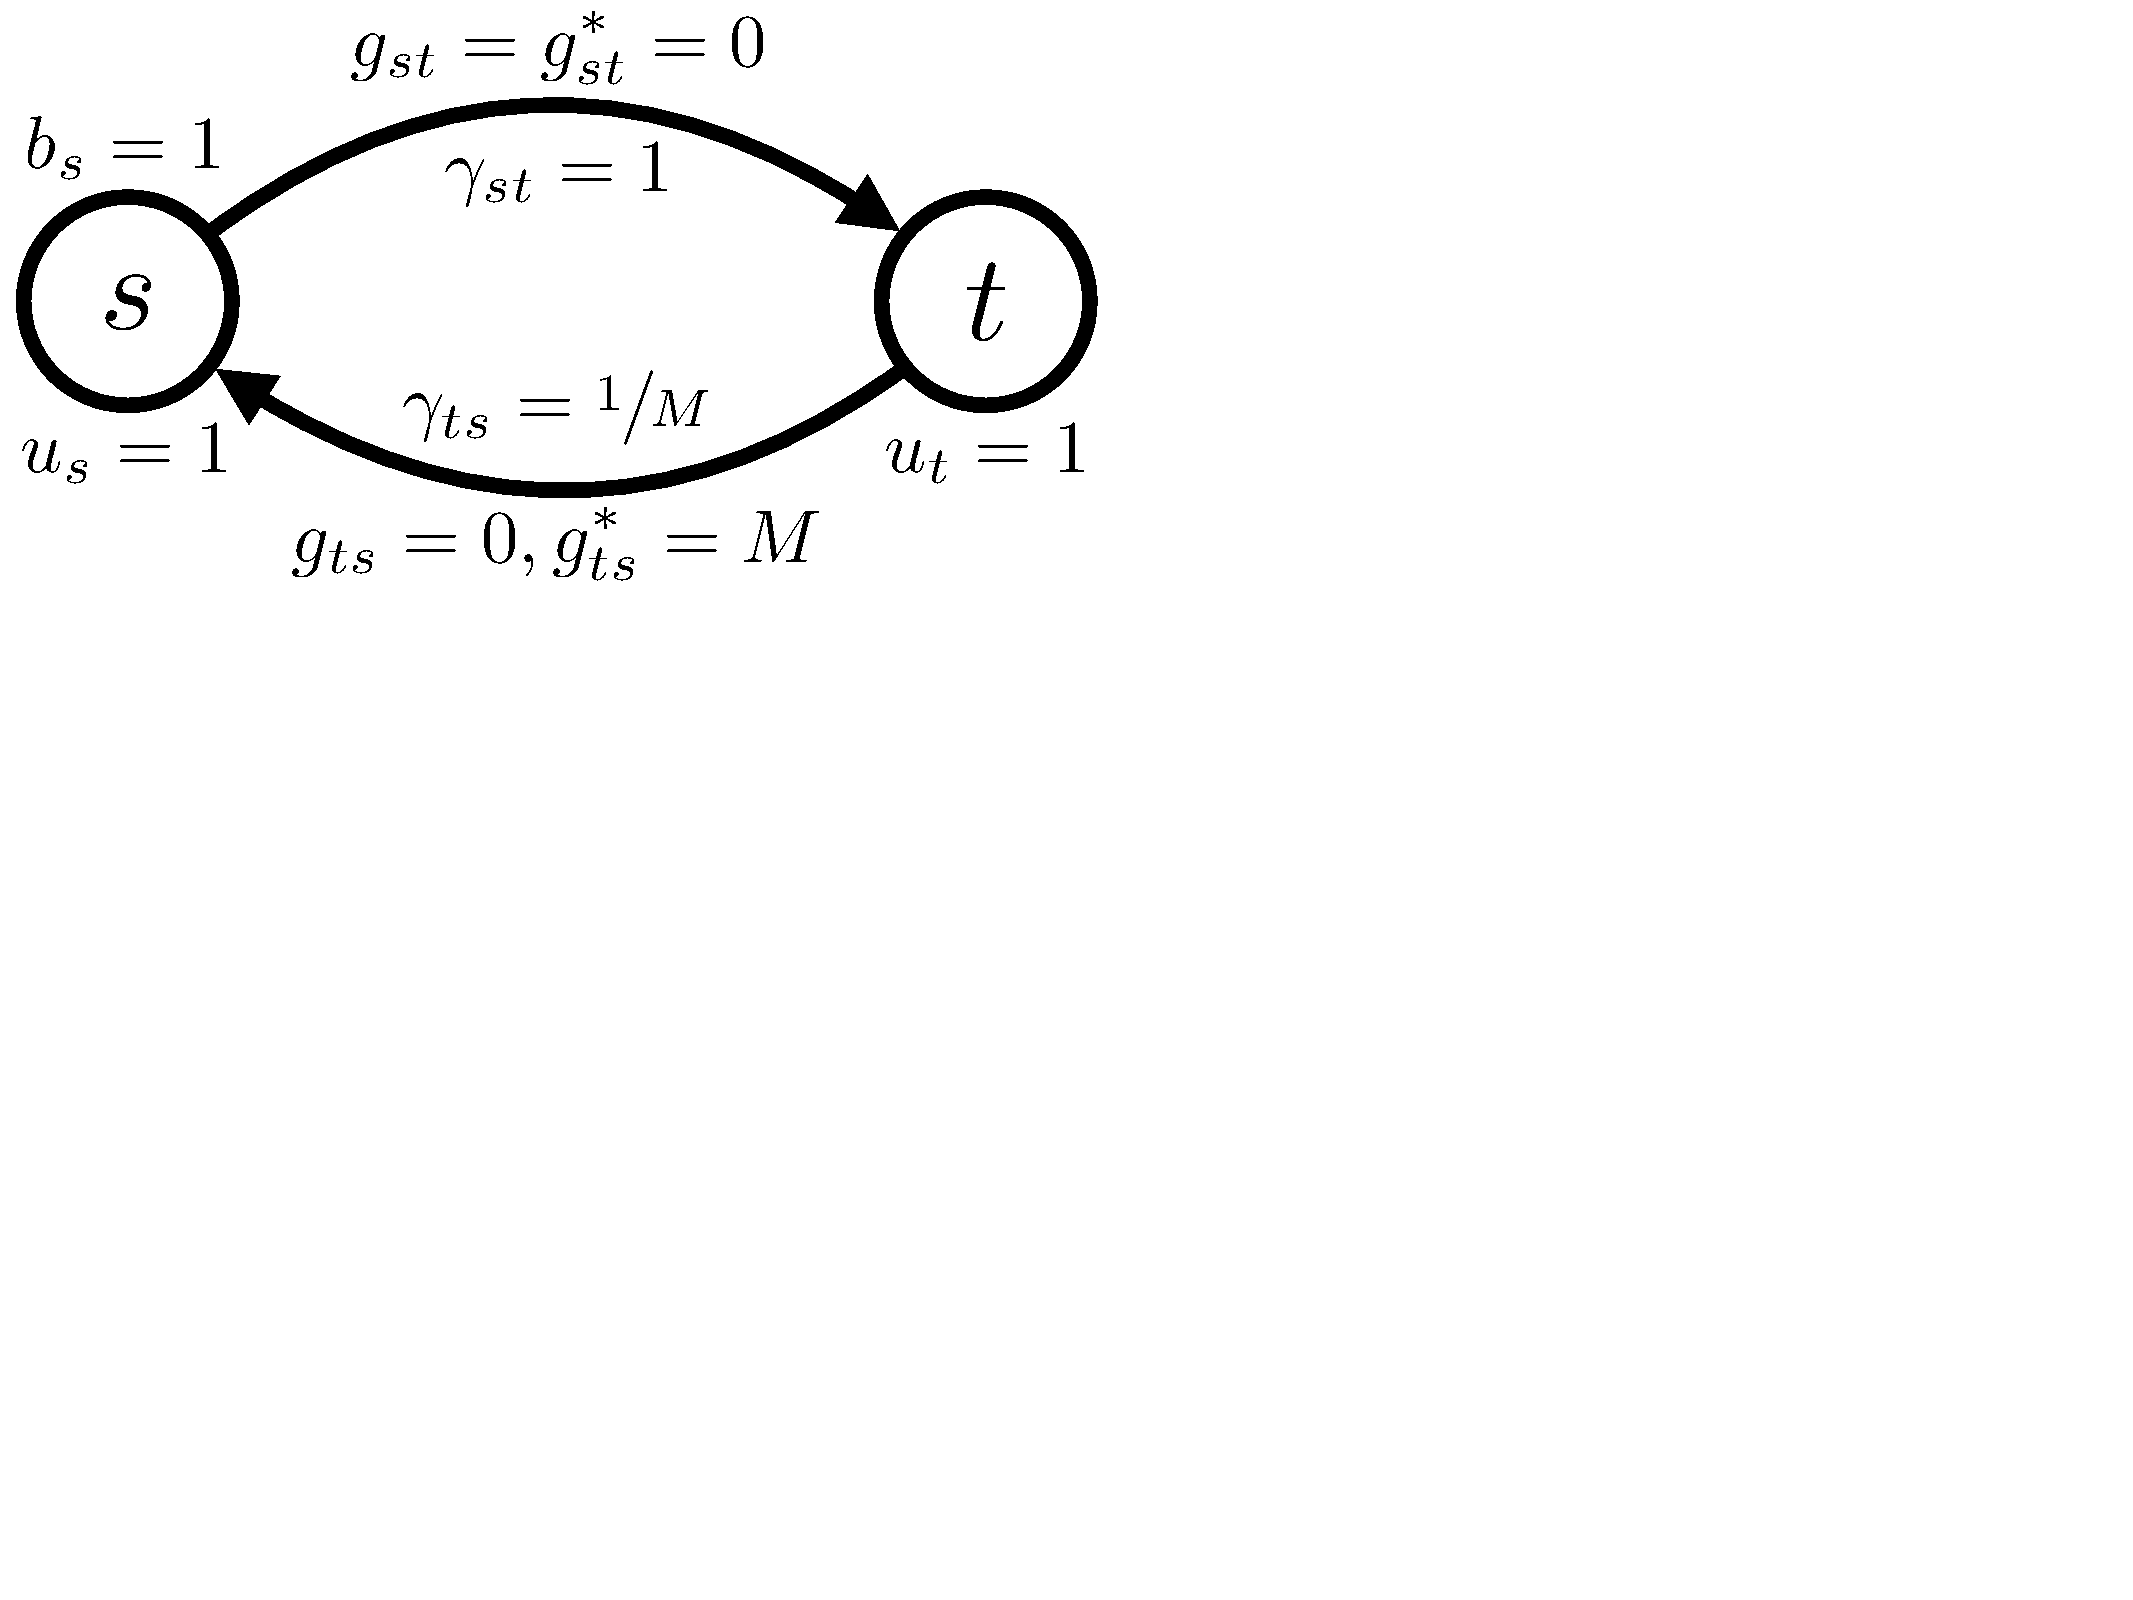
\includegraphics[width=0.45\textwidth]{figs/unsafe.pdf}
    \caption{
    \label{fig:unsafe}
    \rewrite{Simple example showing how unsafe $\mu$ causes problems.}\todo{Keep?}
    }
    \end{figure}

    \subsection{Scaling and Augmentation}
    \label{sec:sub-ppn}
		\todo{Maybe say something about why we don't scale everything. Ideas:
		wouldn't do anything or alpha would have to be 1? Have to be able to send
	the excesses somewhere to have to be conservative and only scale the things
where you can definitely send it}
	The algorithm starts with a feasible fitting pair and consists of a sequence
    of epochs, each dedicated to identifying a contractible edge via a plentiful node.
    Each epoch alternates between the following augmentation and scaling phases:
    \begin{itemize}
    \item \textbf{Augmentation:} Reduce the total excess and deficit of the fitting flow $f$
    by augmenting one unit of flow at a time along tight paths. Formally, let
    $D$ (``destinations'') be the union of the sink $t$ and all nodes with 
    deficit ($\nabla f_i^{\mu} < b_i^{\mu}$). Let $S$ (``sources'') be
    the set of all nodes $i$ for which
    \begin{enumerate}[(i)]
    \item the excess ($\nabla f_i^{\mu} \ge \lceil b_i^{\mu} \rceil$);
    \item $D$ is reachable from $i$ along a tight path in the residual graph; and
    \item $b_i < 0$ (this condition is important in the potential analysis).
    \end{enumerate}
    Augment until $S$ is empty.
    \item \textbf{Scaling:} Once it is not possible to augment any more flow, the second step scales down
    the labels and flow for all nodes and edges in $S$ by the same factor $\alpha$,
    which is chosen to be the largest value that \rewrite{does not violate} any of the dual
    constraints~(D) or produces a plentiful node.
    \end{itemize}

    \todo{RE-WRITE AS DJIKSTRAS}

    Although it is not necessary in practice, for clarify of explanation, one can think of choosing the scaling factor $\alpha$ as solving
    the following LP:
    \lpeq{\lpthree{max}
    {\alpha}
    {\gamma_{ij}^{\mu} \le 1\ \forall\ i,j \in \din(S)}
    {\nfiu - \biu \le 1}
    {\nexists\ \text{plentiful}\ i \in \vsink}
    }
    \begin{figure}[b!]
    \centering
    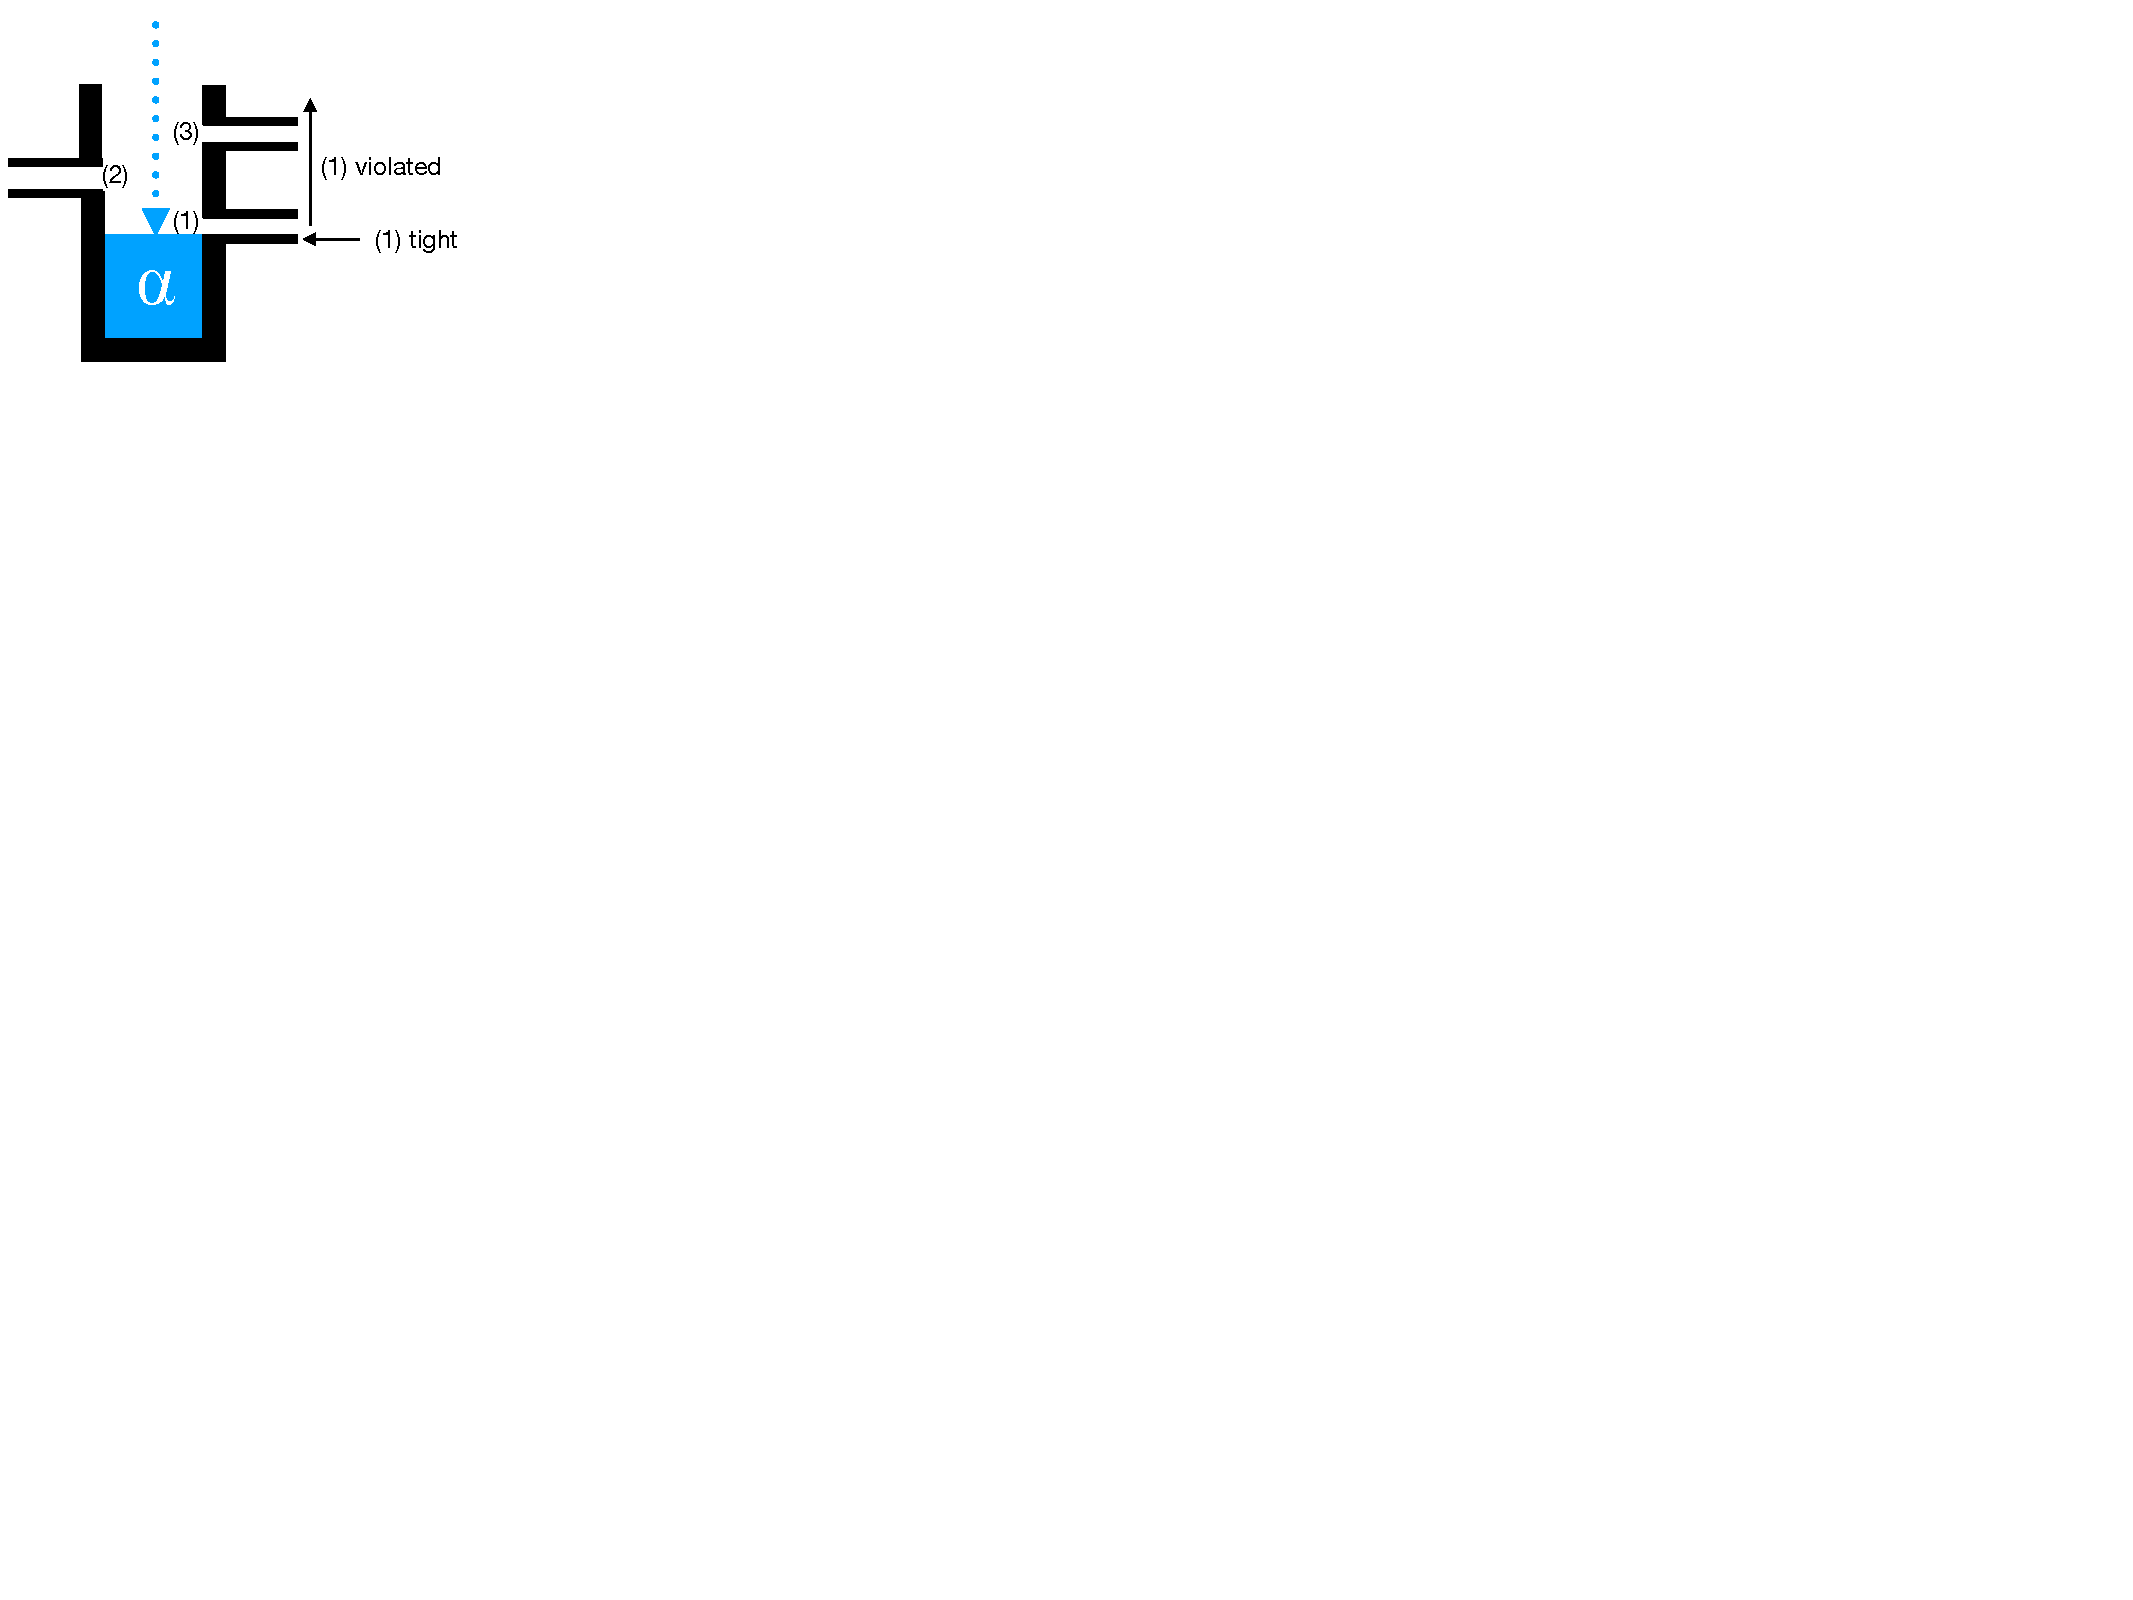
\includegraphics[width=0.35\textwidth]{figs/water.pdf}
    \caption{
    \label{fig:alpha}
    Informal analogy for the maximization of scaling parameter $\alpha$.
    Each pipe represents a constraint. $\alpha$ can only be increased until
    one of them becomes tight as increasing it further would leak into
    the lowest pipe and violate that constraint.
    At each step, the order of which constraint becomes tight first may be different.
    }
    \end{figure}
    Intuitively, as illustrated in Figure~\ref{fig:alpha}, this is akin to filling
    a basin with water as much as possible without any of the water leaking into one
    of three pipes, where each pipe represents a constraint and its height in the basin
    represents the value of $\alpha$ at which point it becomes tight.

    Thus, $\alpha$ is chosen such that one of the following constraints becomes
    tight, or, in other words, one of the following becomes true corresponding to
    each constraint, respectively:
    \begin{enumerate}[itemsep=-1mm]
        \item An edge entering $S$ becomes tight, and thus a new node is added to $S$
        \item A node in $S$ has excess $>1$, which allows us to augment flow from it
        \item A node becomes plentiful
    \end{enumerate}

    If (3) is true, we're done. If (1) or (2) are true, it ensures that we will now
    be able to make progress in the next iteration of the first step. Below, we show
    in Lemma~\ref{lem:scaling} that the augmentations in the first step similarly ensure
    that the algorithm can make progress in the second step. 

    Although it is conceptually easier to imagine increasing $\alpha$ continuously
    until one of these constraints becomes tight, in practice, it is possible to
    calculate $\alpha$ arithmetically in $O(n)$ by picking a value for each node
    that would satisfy one of the tightness conditions and then choosing the minimum
    such value so that only one of the constraints become tight and none are
    violated.
    The details of calculating the value are not particularly insightful so we omit them here, but the
    fact that it can be done is important for the running time analysis.

    We now make some important claims about the variables as the algorithm
    progresses that allow us to prove its correctness: i.e. that it terminates,
    producing a plentiful node.
    In the following section,
    we further prove that it terminates in strongly polynomial time and derive
    an upper bound on the running time.

    \begin{lemma}
    $f^{\mu}$ remains unchanged throughout the subroutine.
    \label{lem:fsame}
    \end{lemma} 
    \begin{proof}
        We must show that, for all edges $(i,j)$, $f_{ij}^{\mu}$ does not change.
        Recall that $f_{ij}^{\mu} = \frac{f_{ij}}{\mu_i}$. There
        are four possible cases for $(i, j)$:
        \begin{enumerate}
            \item Both outside of $S$. The subroutine only scales $i \in S$, so $\mu_i$ 
                does not change, and thus nor does $\fiju$.
            \item Both inside of $S$. The subroutine scales both $f_{ij}$ and $\mu$ by
                $\alpha$, which cancel each other out in the definition of $\fiju$.
            \item Only $i$ in $S$, which implies $i,j \in \dout(S)$. Then $f_{ij}=0$,
                because otherwise there would be a tight residual edge $j,i \in \din(S)$,
                and by definition $S$ has no incoming tight edges.
            \item Only $j$ in $S$, which implies $i,j \in \din(S)$. Again, incoming edges
                are not tight by definition of $S$ and we only augment along tight edges,
                so $f_{ij}$ is not augmented. Also, if $i \notin S$, then $\mu_i$ doesn't
                change. \qedhere
        \end{enumerate}
    \end{proof}
    \begin{corollary}
    $f^{\mu}$ is always integral.
    \end{corollary}
    \begin{proof}
    The augmentation step clearly maintains integrality of $f^{\mu}$ because we
    always augment by 1 unit at a time. The only other part of the algorithm that
    modifies the primal solution is the relabeling of $f_e$, and by
    Lemma~\ref{lem:fsame}, this never changes the value of $f^{\mu}$.
    \end{proof}
    \begin{lemma}
        \label{lem:scaling}
        For all nodes with non-zero demand in $S$, scaling $\mu$ in the second step
        strictly increases $|\biu|$. For all other nodes, $|\biu|$ remains unchanged.
        \todo{Show S cannot be empty?}
    \end{lemma}
    \begin{proof}
        First, trivially, scaling a node with zero demand cannot change its value
        ($0\cdot\mu=0$), and the algorithm only updates $\mu_i$ for $i \in S$. Recall
        that $\biu$ is defined as $b_i / \mu_i$, and thus, if $\mu_i\leftarrow \mu_i / \alpha$,
        then
        \[ \biu \leftarrow \frac{b_i}{\mu_i / \alpha} = \alpha\frac{b_i}{\mu_i} = \alpha \biu. \] 
        Now it suffices to prove that $\alpha > 1$ always holds when any of the three
        constraints become tight.

        By construction, before rescaling, $S$ has no tight
        incoming edges. Recall $\giij = \gamma_i\frac{u_i}{u_j}$. In order for an
        incoming edge $i \notin S, j\in S$ to become tight (1), we must have $\giij=1$:
        since we only scale values in $S$, $\alpha$ must be ${1}/{\giij}$, which is
        always greater than $1$ because $\giij < 1$ (by the feasibility of the dual).

        From the terminating condition of the augmentation step (the lack of any nodes
        in $S$ having excess), we know $\Ex(f) = \nfiu - \biu < 1$. Since, by
        Lemma~\ref{lem:fsame}, $\nfiu$ is unchanged and only nodes in $\vsrc$ (i.e. $b_i<0$)
        can have excess, the only way for to make $\Ex(f) \ge 1$ is if $\biu$ becomes
        more negative, which only happens if $\alpha > 1$. 

        Finally, we start out with the assumption that there are no plentiful nodes.
        In order for a node to become plentiful (3), its demand $\biu$ must increase,
        which is only possible if $\alpha > 1$.
    \end{proof}
    \begin{lemma}
        \label{lem:still-fit}
        $\fp$ remains a fitting pair throughout the subroutine.
    \end{lemma}
    \begin{proof}
        In order to be a fitting pair, we must have the following relationship between
        $f$ and $\mu$: for all $(i, j) \in E$, $\giij \leq 1$, and when $f_{ij} > 0$, 
        $\giij = 1$. \todo{This is a definition, not a proof.}
    \end{proof}

    \begin{lemma}
        The rescaling of $\mu$ during produce-plentiful-node does not break 
        the safety of $\mu$, i.e. there is a corresponding feasible primal
        solution even though we haven't kept track of it.
        \todo{Why is this here:} (~\ref{lem:usafe})
    \end{lemma}
    \begin{proof}
    The initialization subroutine is guaranteed to produce a fitting pair $\fp$,
    where $f$ is feasible, so we have that initially $\mu$ is safe. Now assume $\mu$
    is safe before running the subroutine. For sake of contradiction, assume that
    after running the subroutine, the updated labeling $\mu'$,
    is no longer safe. That is, there exists some subset of nodes $X \subseteq \vnott$  
    without any incoming tight edges ($\{\gamma_e^{\mu'} = 1\ \forall\ e \in \din(X)\} = \varnothing$)
    and where all nodes have positive demand $b^{\mu'}(X) > 0$.

    Suppose we divide $X$ into two parts: the subset of nodes in $S$, $X \cap S$, and those
    not in $S$, $X \setminus S$. Recall that $\mu_i' = \frac{\mu}{\alpha}$ for $i\in S$
    and $\mu' = \mu$ for $i \notin S$. Then we can rewrite the node demands under $\mu'$
    in terms of the demands under $\mu$ as follows:
    $$b^{\mu'}(X) = \frac{1}{\alpha}b^{\mu}(X \cap S) + b^{\mu}(X \setminus S)$$
    If, as we assumed, $b^{\mu'}(X) > 0$, then either $b^{\mu}(X \cap S)$ or 
    $b^{\mu}(X \setminus S)$ must be positive.
    \todo{Fill in details. $\mu'$ is defined in terms of $S$.}
    Now consider the set of edges coming into each of these subsets...
    Any edge that's tight under $\mu'$ was tight under $\mu$, because $\geu$, if
    it has no tight edges under $\mu'$ then it also had no tight edges under
    $\mu$.

    Therefore, since neither of the two parts of $X$
    have any tight incoming edges under $\mu$ and at least one of them
    must have strictly positive node demands, at least one of them
    violates the safety conditions of $\mu$ and thus $\mu$ was not safe.
    This is a contradiction, and thus if $\mu$ was safe, $\mu'$ must also be safe.

    \end{proof}

    In summary, we have shown that the primal and dual steps always allow room for the other to make progress, and collectively each iteration of the two steps strictly increases $|\biu|$ towards
    the definition of a plentiful node. Thus, the subroutine will eventually produce one. We have also shown that the updates it makes to $f$ and $\mu$ do not violate any of the previous conditions stated for being able to ultimately derive a primal optimal solution once our fitting pair finds the dual optimal. 

\iffalse
	 \subsection{Finding a feasible flow}
	\todo{Don't they just run the whole algorithm on a modified graph to initialize?}
	Drawing inspiration from the Simplex algorithm, the first step in this algorithm is finding a trivial feasible solution $(\bar{f}, \bar{\mu})$, which clearly also satisfies the definition of a fitting pair necessary for the algorithm. In order to find this initial solution, rather than using Radzik's cycle-cancelling subroutine as in prior work, the authors develop a new method based on negative cycle detection, which can be run in $O(nm)$ time. \todo{references} 
    \fi
    
    \subsection{Scaling and Rounding} 
    Since the second phase of the algorithm relies on the relabeled flow, $f^\mu$, being integral, we must first round the initial feasible flow (which does not have an integrality constraint) and then maintain its integrality throughout the second phase until finding the final optimum. Using the integrality properties of maximum flow, we can run a feasible circulation problem on the relabeled graph to find an integral max flow. We do this by taking the initial fitting pair $(f, \mu)$ and corresponding feasible relabeled flow $f^\mu$ and setting a lower bound of $\lfloor \nabla f_i^\mu \rfloor$ and an upper bound of $\lceil \nabla f_i^\mu \rceil$. The corresponding integral relabeled max flow on each edge $(i, j)$ can be turned into an integral flow by multiplying by $\mu_i$. Throughout the second phase, the value of $f_{ij}^\mu$ remains unchanged because if $f_{ij}$ is scaled, the algorithm scales $\mu_i$ by the same amount; therefore, $f_{ij}^\mu$ remains integral after the initial rounding.
    
    In addition to rounding the initial feasible flow, the initial labels, $\mu$, are scaled at the beginning of phase 2. Before rounding, we set a scaling factor $\Delta$ equal to $\max_{i \in V \setminus t} \nfiu - \biu$, which is the maximum excess at a node in the initial feasible solution. We multiply $\mu$ by $\Delta$, which reduces $f^\mu$ by a factor of $\Delta$. This scaling is useful because it bounds $\nfiu$, which is used to bound the total excess in the amortized analysis (explained in Section 5.8). The resulting bound is $\biu - 1 \leq \nfiu \leq \biu + 2$ for all $i \in V \setminus t$; the derivation leading to this result is not explicitly explained in the original paper \cite{Olver2017}, but we provide a clearer explanation. Initially, $\nfiu \geq \biu$ because it must be feasible. After rounding, $\nfiu \geq \biu - 1$ because $\nfiu$ decreases by at most $1$ during rounding. This gives the lower bound of the result. The upper bound comes from the scaling and the definition of $\Ex(f, \mu)$ in Section~\ref{sec:lp}. Since we scale $\nfiu$ down by the maximum excess in the initial solution, the maximum in $\Ex(f,\mu)$ will never be more than $2$. This gives the upper bound $\nfiu \leq \biu + 2$. 

    \subsection{Running Time Analysis}
    The algorithm consists of three basic types of operations: scaling, augmentation, and contraction.
    The number of contractions is bounded by $n$. Contraction itself
    requires computing a regular flow and performing a bounded number of graph operations, but
    strongly polynomial algorithms already exist for these. So the goal is to bound the running time
    (number of arithmetic operations) between any two contractions.

    Augmentation itself consists of a graph search on the tight subgraph, an $O(m)$ operation.
    Between rounds of augmentation, there is a scaling round. Each atomic scaling step stops
    when either (i) a node has become plentiful, leading to a contraction; (ii) a node has an
    excess greater than $1$, leading to a new augmentation round; or (iii) the loose cut
    $S$ has been extended by at least one node. (iii) can only happen at most $n$ times; thus,
    there are at most $n$ scaling steps between any two augmentations. Each scaling step
    is an $O(n)$ operation, leading to a naive time bound of $O(n^2)$ between any two augmentations.
    This can be improved to $O(m + n \log n)$ by applying the framework of Dijkstra's
    algorithm with costs $-\log \gamma^u_e$. The loose cut $S$ corresponds to the expanding
    frontier of Dijkstra's algorithm.

    It remains to bound the total number of augmentations the algorithm may perform. We'd
    like to show that after a strongly polynomial number of augmentations, the algorithm
    is guaranteed to find a plentiful node.

    \begin{lemma} \label{lem.num-aug}
        After $O(mn)$ augmentations, the algorithm is guaranteed to find a plentiful node.
    \end{lemma}
    First, a preliminary lemma. We denote the period between successive contraction
    steps as an epoch.
    \begin{lemma}
    At any node $i \in \vsrc$, the deficit is at most one. Moreover, at most one augmentation
    ends at such a node during any epoch.
    \end{lemma}
    \begin{proof}
        At the beginning of the algorithm, the flow is feasible, so $\nfiu - \biu \geq 0$.
        Rounding decreases $\nfiu$ by less than one. Similarly, during each contraction,
        the adjusted flow is computed with $nabla g_i^\mu \geq \lfloor \biu \rfloor$ everywhere.

        Between contractions, the deficit can be modified by scaling and augmentation steps.
        Since $i \in \vsrc$, $\biu < 0$, and so $\biu$ can only decrease during scaling.
        Meanwhile, augmentations only decrease deficits.
        Once $\nfiu \geq \biu$, no augmentation ending at $i$ will be contemplated unless $i$
        experiences a deficit again. The only way for this to happen would be for
        augmentations beginning at $i$ to reduce $\nfiu$ below $\biu$. However,
        an augmentation will only begin at $i$ if
        $\nfiu - \biu \geq 1$, and will reduce $\nfiu$ by exactly one. Hence, $i$ will
        never again experience a deficit during the epoch, and so there will be no further
        augmentations ending at $i$.
    \end{proof}

    \begin{proof}[Proof of Lemma \ref{lem.num-aug}]
    Define two potential functions
    \begin{align*}
    \Psi(\mu) &= - \sum_{i \in \vsrc} \biu \\
    \Phi(\mu) &= \sum_{i \in \vsrc} \nfiu + \Psi(\mu) = \sum_{i \in \vsrc} \nfiu - \biu
               \leq \Ex(\mu)
    \end{align*}
    \todo{complete proof}
    \end{proof}


\section{Discussion and Future Work}\label{sec:discussion}

	\subsection{Non-triviality of a strongly polynomial algorithm}

	\todo{Explain} why applying ideas from strongly polynomial algorithms for
	min-cost flow was not straightforward. 

	We know that the feasibility problems are the same for min-cost and
	generalized max-flow. Min-cost objective is additive: when you change the
	value of the flow on one edge, that doesn't affect the objective piece for any
	other edge, whereas in the
    
    %feedback 
    \vspace{10mm}
\todo{Main feedback from emails:} 

\todo{(1) more "english descriptions" for safe sets and loose cuts}

\todo{(2) too many definitions}

\todo{(3) paper needs more synthesis and should have explicit outline and more main ideas rather than full proofs}

\todo{(4) make $\Delta$-scaling part more clear}

\todo{(5) Section 4 too definition heavy; needs more intuition}

\todo{(6) intuition for why taking dual helps}

	%feedback

\setlength{\bibitemsep}{0pt}
\nocite{*}
\printbibliography
\end{document}
 
